\section{Correlazione}
In questo capitolo si analizza la relazione presente tra le diverse variabili tramite la matrice di correlazione.

\noindent
La matrice di correlazione mette in mostra la correlazione tra ogni coppia di variabili del dataset, per questo motivo otteniamo una matrice simmetrica.

\noindent
In questo caso abbiamo sull'anti-diagonale l'incrocio con la stessa identica variabile e questo comporta la correlazione massima.

\noindent
In seguito sono riportate le matrici di correlazione [\ref{fig:correlation_O}], [\ref{fig:correlation_NoO}] dove la seconda matrice mostra i dati dopo aver tolto gli outliers dal dataset .

\noindent
I valori positivi di correlazione indicano che all'aumentare dei valori di una variabile aumentano anche i valori assunti dall'altra variabile, mentre i valori di correlazione negativi indicano che al crescere dei valori di una variabile corrisponde un andamento di decrescita nei valori dell'altra variabile.

\noindent
Come si può notare otteniamo una correlazione molto bassa, questo conferma quanto precedentemente affermato riguardo alla difficoltà per un modello di poter inferire sui dati.

\noindent
Osservando i valori di correlazione che caratterizzano la variabile \textit{quality} si può notare come solo \textit{alcohol} e \textit{volatile.acidity} forniscono una correlazione utile per poter distinguere la classe di qualità, ma comunque con valori medio bassi e quindi poco significativi.

\noindent
Inoltre questa bassa correlazione suggerisce che l'utilizzo di una PCA non porterà a miglioramenti significativi.

\noindent
Come si può notare osservando i due grafici la rimozione degli outliers porta a piccoli miglioramenti aumentando la correlazione in valore assoluto.

\newpage

\begin{figure}[H]
    \centering
    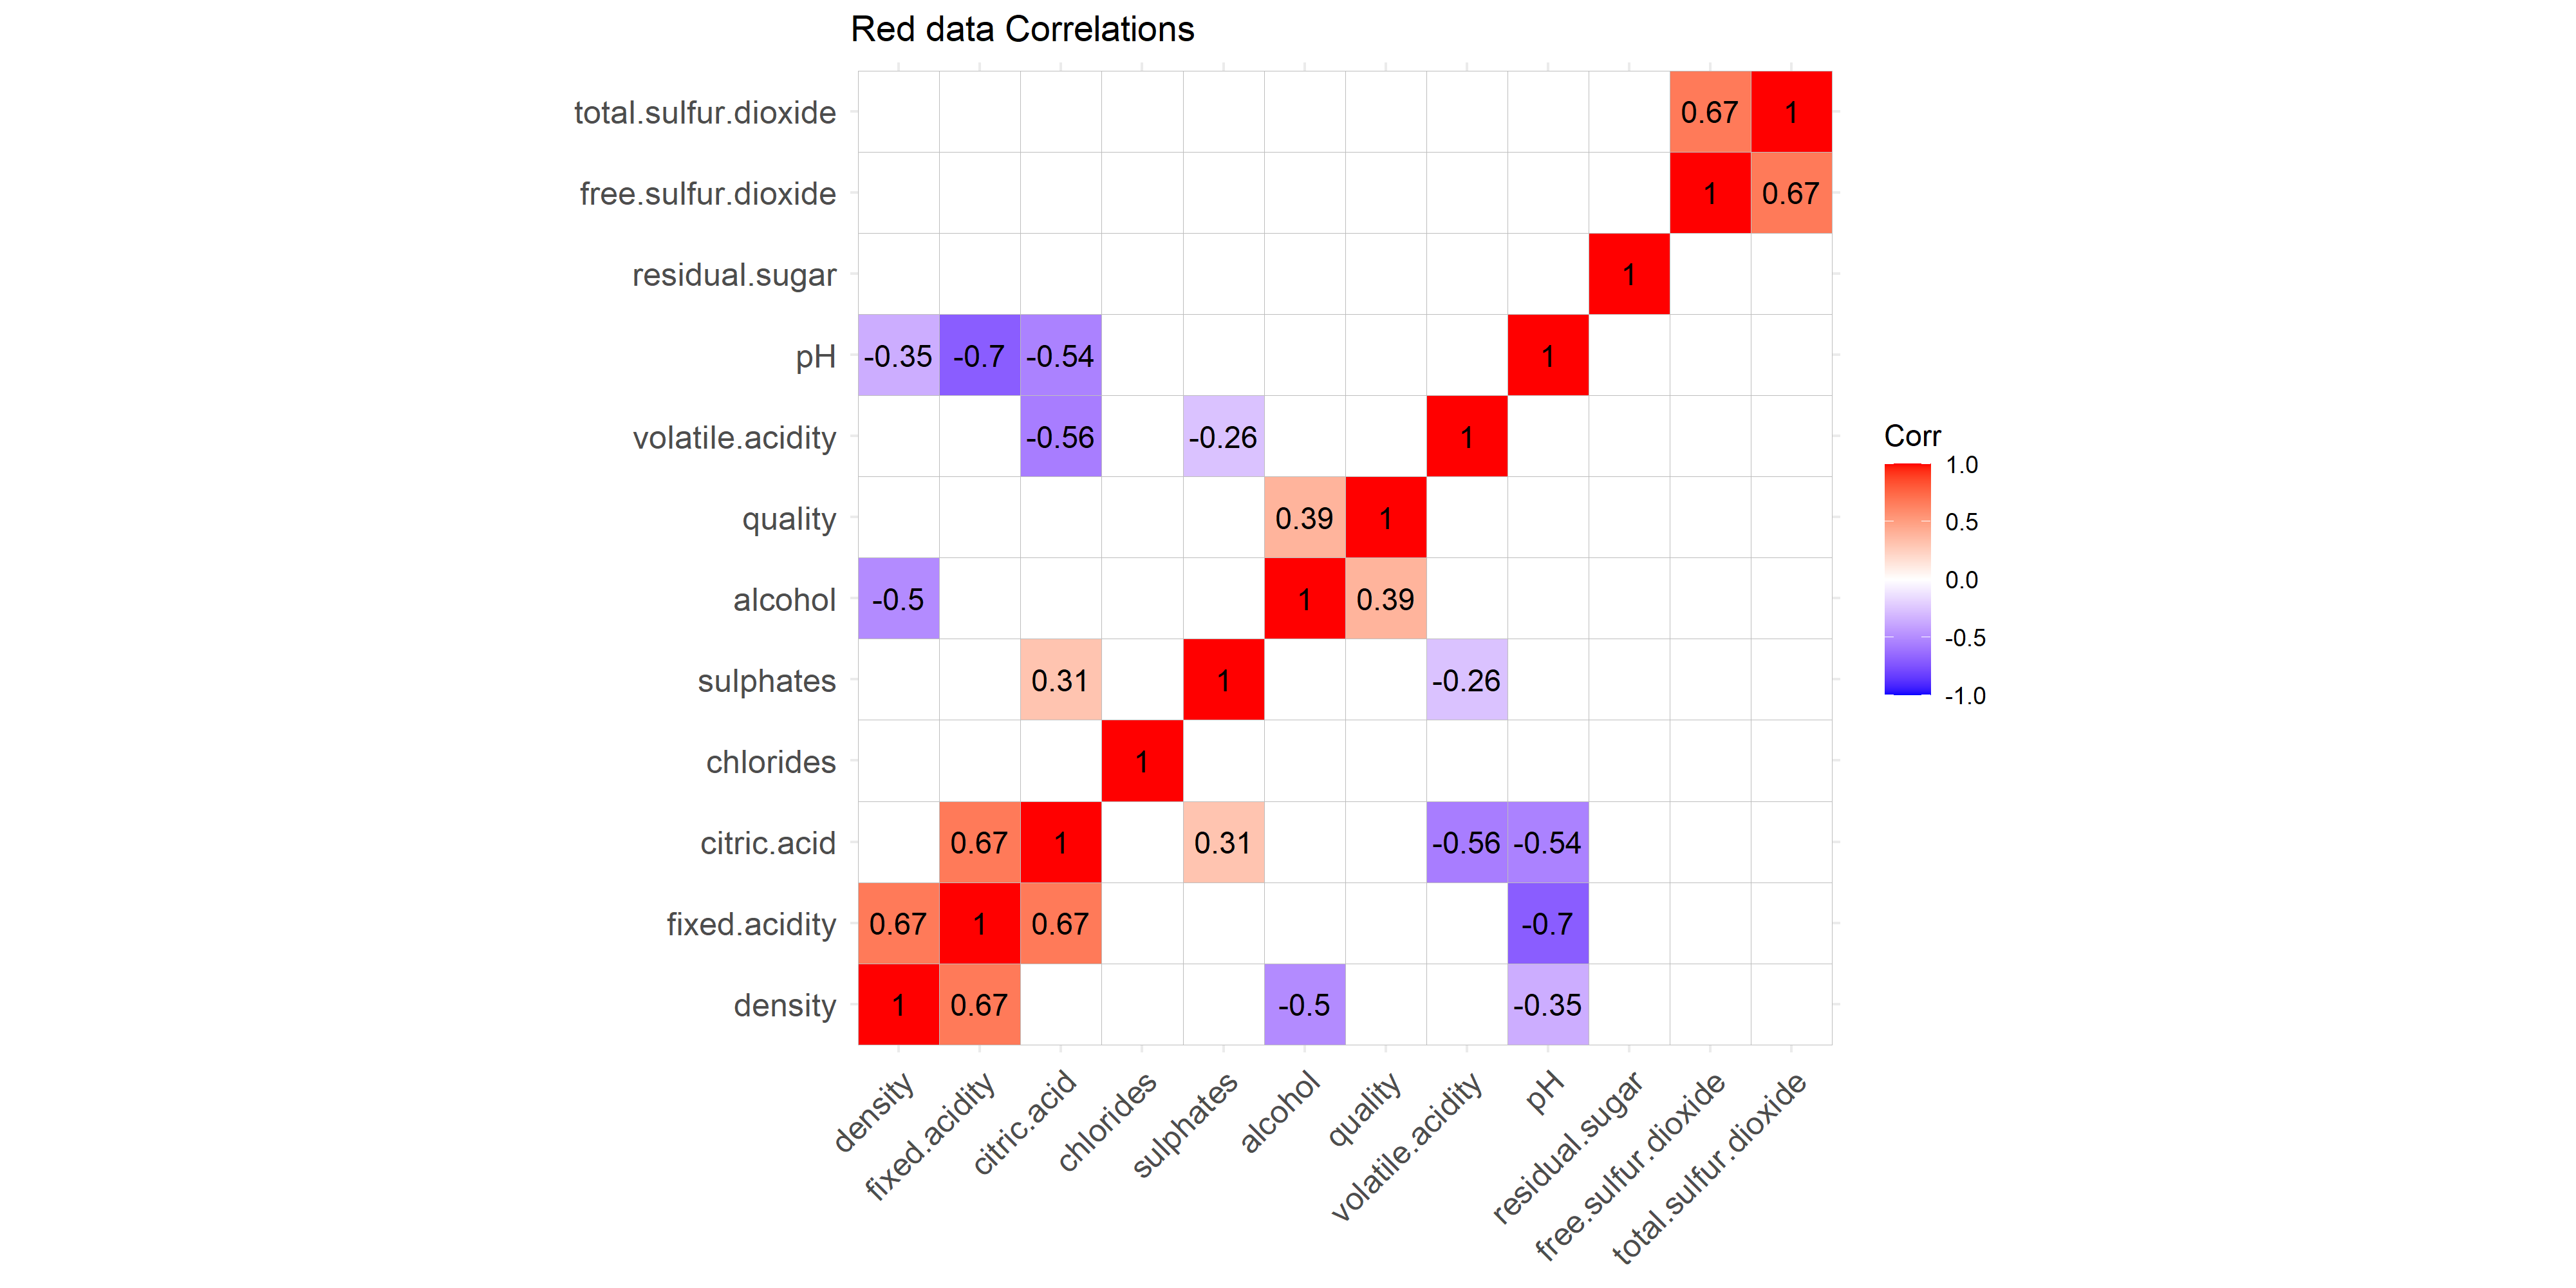
\includegraphics[scale=.5]{images/analisi/correlazione/Correlation_matrix_.pngO.png}
    \caption{Questa immagine rappresenta una matrice della correlazione che mette in evidenza le maggiori correlazioni tra le diverse variabili.}
    \label{fig:correlation_O}
\end{figure}

\begin{figure}[H]
    \centering
    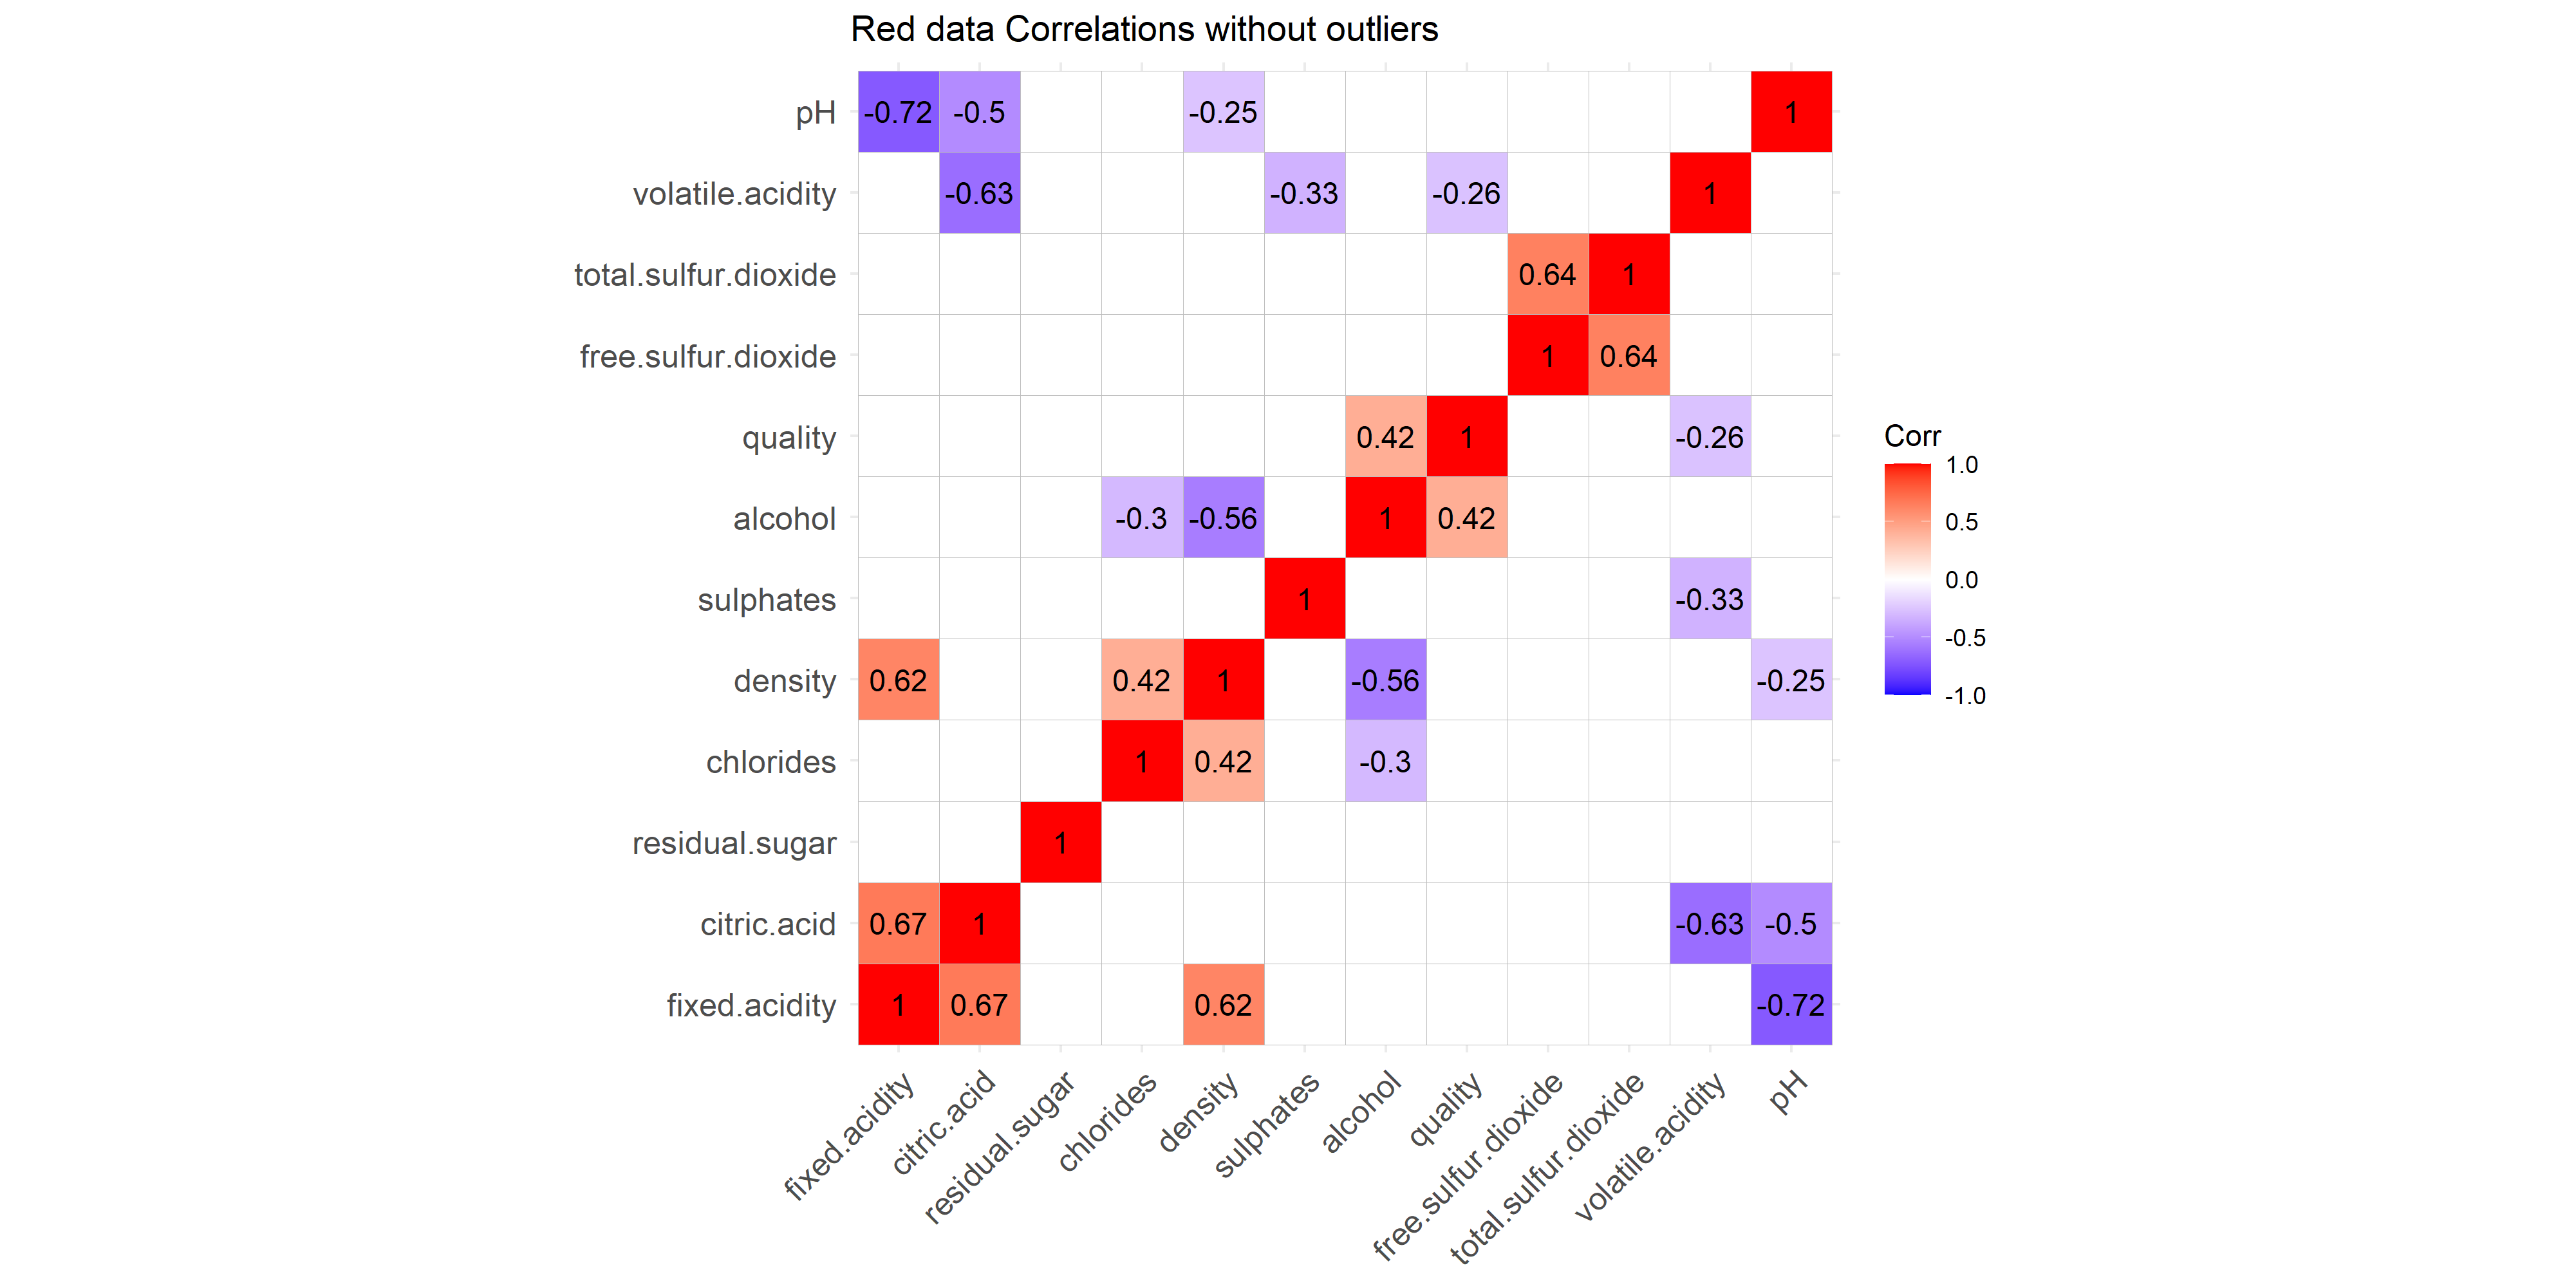
\includegraphics[scale=.5]{images/analisi/correlazione/Correlation_matrix_.pngNoO.png}
    \caption{Questa immagine rappresenta una matrice della correlazione che mette in evidenza le maggiori correlazioni tra le diverse variabili, in questo specifico caso il dataset non contiene gli outlier.}
    \label{fig:correlation_NoO}
\end{figure}
